%auto-ignore
\section{Results}
\label{sec:results}
We train a number of base Transformer models at different parameter sizes, ranging from 600M to 3B parameters. Each of these models is fed in the output embeddings from a T5-XXL model, which is pre-trained and frozen and consists of 4.6B parameters. Our largest base model of 3B parameters consists of $48$ Transformer layers with cross-attention from text to image and self-attention among image tokens. All base models share the same image tokenizer. We use a CNN model with $19$ ResNet blocks and a quantized codebook of size $8192$ for the tokenization. Larger codebook sizes did not result in performance improvements. %We also finetuned the decoder, as outlined in \secc{dec_finetune}, replacing the original decoder with\jarred{update} ZZ more convolutional layers and finetuning. Finally,
The super-resolution model consists of $32$ multi-axis Transformer layers~\cite{hit} with cross-attention from concatenated text and image embedding to high resolution image and self-attention among high resolution image tokens. This model converts a sequence of tokens from one latent space to another: the first latent space being that of the base model tokenizer, a latent space of $16\times16$ tokens, to that of a higher resolution tokenizer with $64\times64$ tokens. After token conversion, the decoder for the higher resolution tokenizer is used to convert to the higher resolution image space. Further details of configurations are provided in the appendix.

We train on the Imagen dataset consisting of 460M text-image pairs \citep{imagen}.
Training is performed for 1M steps, with a batch size of 512 on 512-core TPU-v4 chips \citep{jouppi2020domain}. This takes about 1 week of training time. We use the Adafactor optimizer \citep{shazeer2018adafactor} to save on memory consumption which allowed us to fit a 3B parameter model without model parallelization. We also avoid performing exponential moving averaging (EMA) of model weights during training, again to save on TPU memory. In order to reap the benefits of EMA, we checkpoint every 5000 steps, then perform EMA offline on the checkpointed weights with a decay factor of 0.7. These averaged weights form the final base model weights.

\begin{figure}
  \centering
  \begin{tabular}{p{25mm}p{25mm}p{25mm}|p{25mm}p{25mm}p{25mm}}
    \multicolumn{3}{c}{Cardinality} &
    \multicolumn{3}{c}{Composition}
    \\
    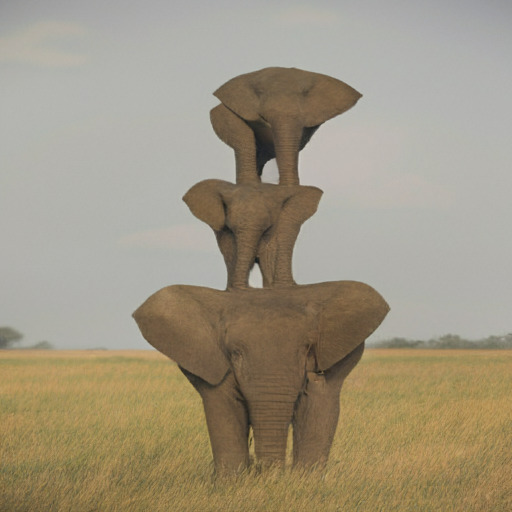
\includegraphics[width=26mm]{figs/verticals/cardinality_00430_maskgit_sresg1r1} &       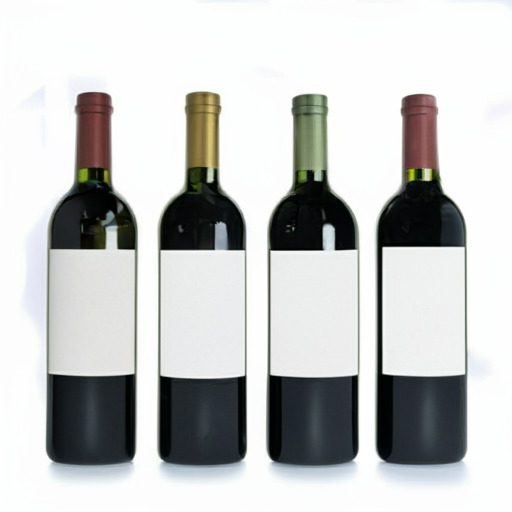
\includegraphics[width=26mm]{figs/verticals/cardinality_00708_maskgit_sresg1r1} &
    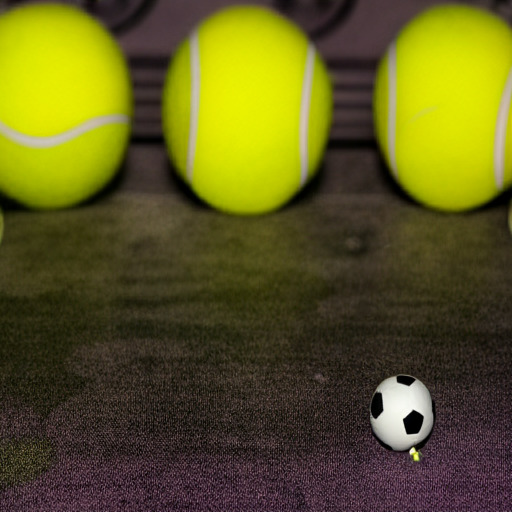
\includegraphics[width=26mm]{figs/verticals/cardinality_00087_maskgit_sresg1r1} &
    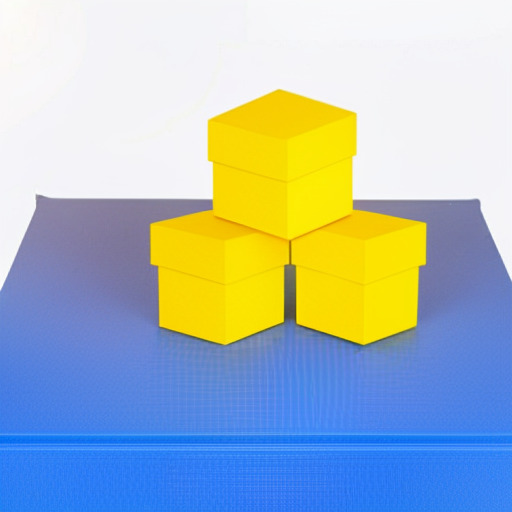
\includegraphics[width=26mm]{figs/verticals/composition_00678_maskgit_sresg1r1} &
    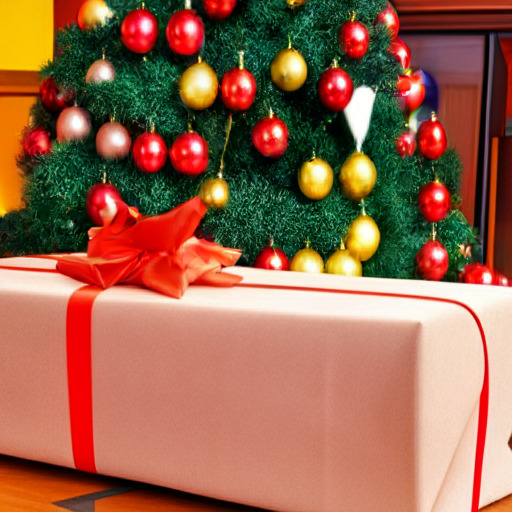
\includegraphics[width=26mm]{figs/verticals/composition_00681_maskgit_sresg1r1} &
    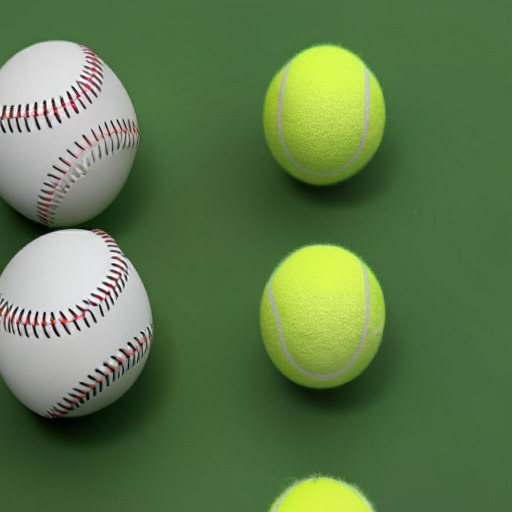
\includegraphics[width=26mm]{figs/verticals/composition_01426_maskgit_sresg1r1}
    \\
    \tiny Three elephants standing on top of each other. &
    \tiny Four wine bottles. &
    \tiny A tiny football in front of three yellow tennis balls. &
    \tiny Three small yellow boxes on a large blue box. &
    \tiny A large present with a red ribbon to the left of a Christmas tree. &
    \tiny Two baseballs to the left of three tennis balls.
    \\
    \noalign{\vskip 2mm}
    \multicolumn{3}{c}{Style} &
    \multicolumn{3}{c}{Text Rendering}
    \\
    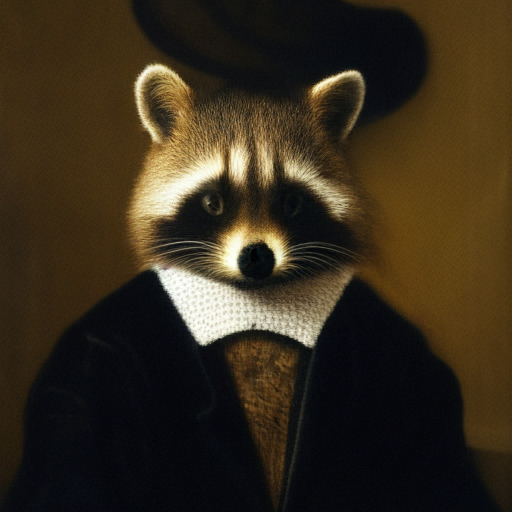
\includegraphics[width=26mm]{figs/verticals/style_00020_maskgit_sresg1r1} &
    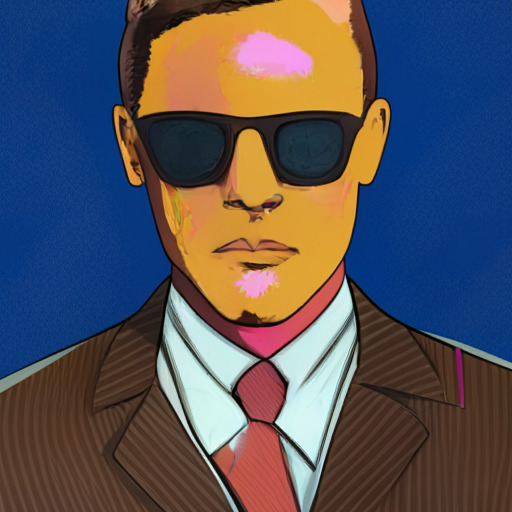
\includegraphics[width=26mm]{figs/verticals/style_00022_maskgit_sresg1r1} &
    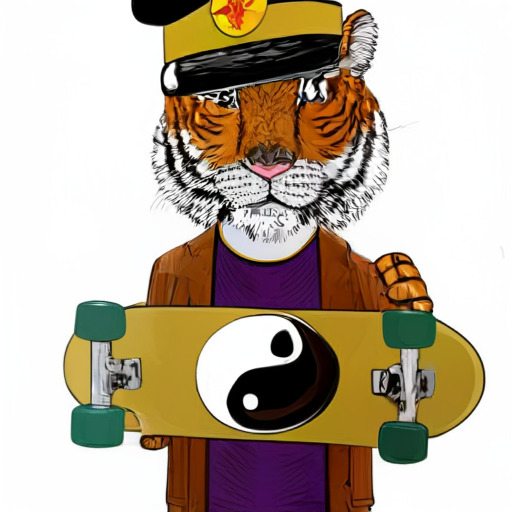
\includegraphics[width=26mm]{figs/verticals/style_01342_maskgit_sresg1r1} &
    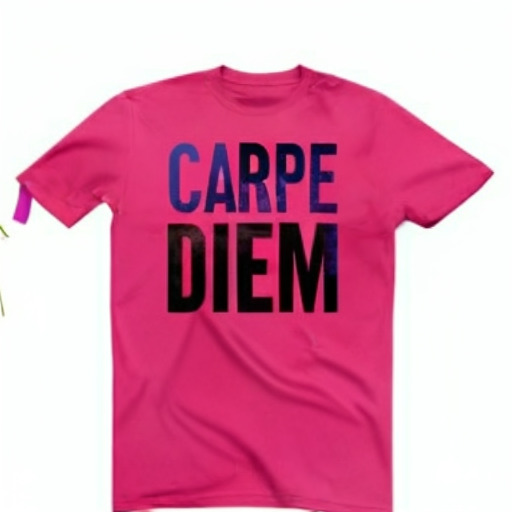
\includegraphics[width=26mm]{figs/verticals/text_00716_maskgit_sresg1r1} &
    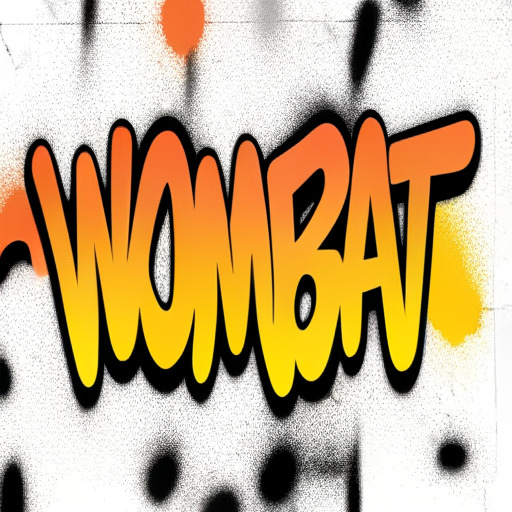
\includegraphics[width=26mm]{figs/verticals/text_01470_maskgit_sresg1r1} &
    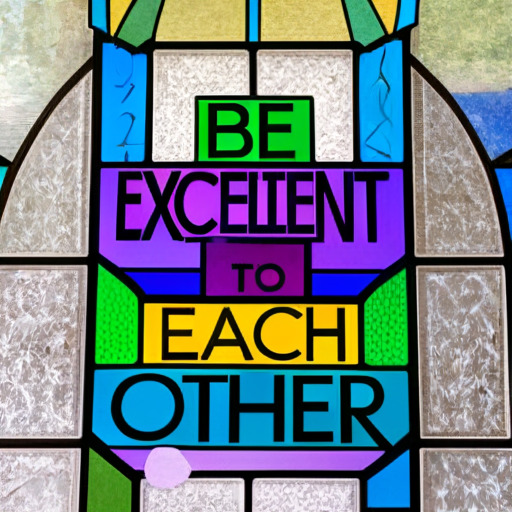
\includegraphics[width=26mm]{figs/verticals/text_01494_maskgit_sresg1r1}
    \\
    \tiny Portrait of a well-dressed raccoon, oil painting in the style of Rembrandt. &
    \tiny A portrait of a man wearing sunglasses and a business suit, painting in pop art style. &
    \tiny Portrait of a tiger wearing a train conductor’s hat and holding a skateboard that has a yin-yang symbol on it. Chinese ink and wash painting. &
    \tiny A t-shirt with Carpe Diem written on it. &
    \tiny High-contrast image of the word ``WOMBAT'' written with thick colored graffiti letters on a white wall with dramatic splashes of paint. &
    \tiny The saying ``BE EXCELLENT TO EACH OTHER'' written in a stained glass window.
    \\
    \noalign{\vskip 2mm}
    \multicolumn{3}{c}{Usage of Entire Prompt} &
    \multicolumn{3}{c}{Failure Text Classes}
    \\
    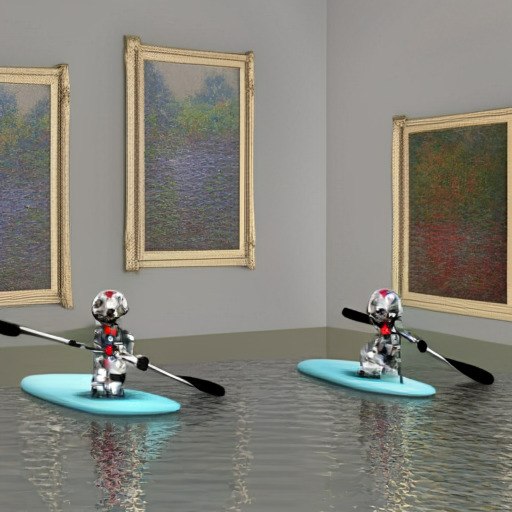
\includegraphics[width=26mm]{figs/verticals/detail_00030_maskgit_sresg1r1} &
    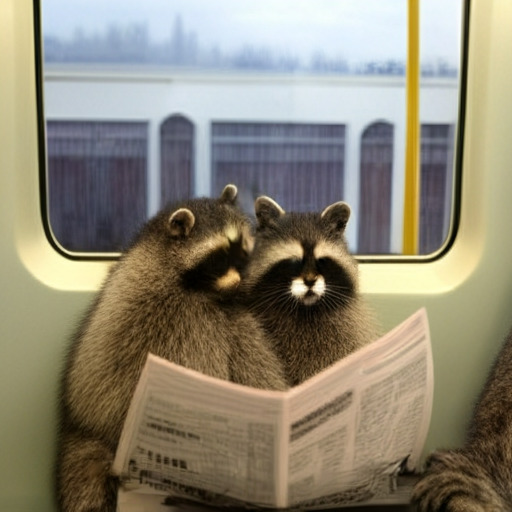
\includegraphics[width=26mm]{figs/verticals/detail_01370_maskgit_sresg1r1} &  
    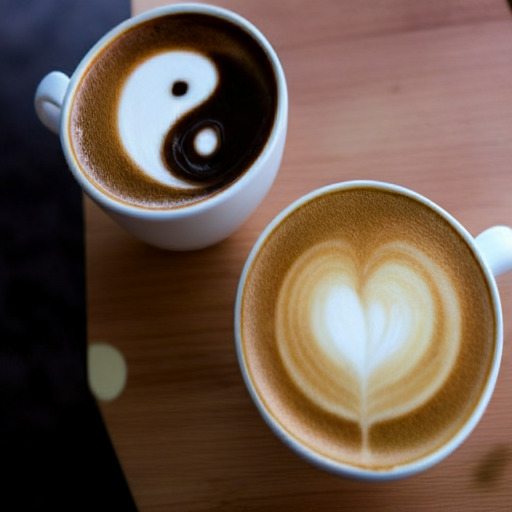
\includegraphics[width=26mm]{figs/verticals/detail_01459_maskgit_sresg1r1} &
    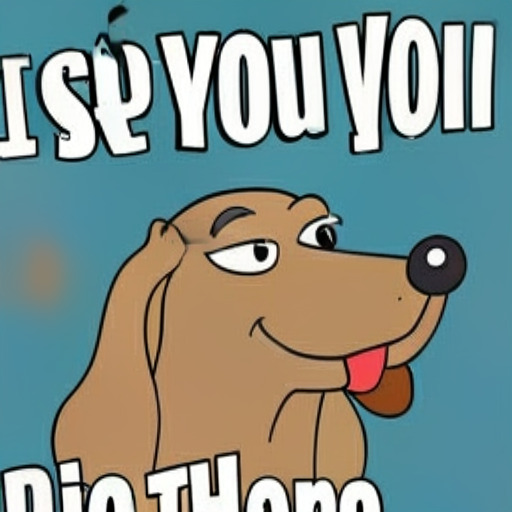
\includegraphics[width=26mm]{figs/failures/failure_00036_maskgit_sresg1r1} &
    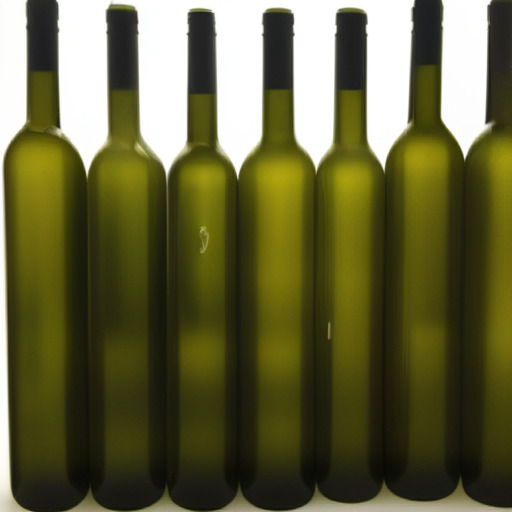
\includegraphics[width=26mm]{figs/failures/failure_00709_maskgit_sresg1r1} &
    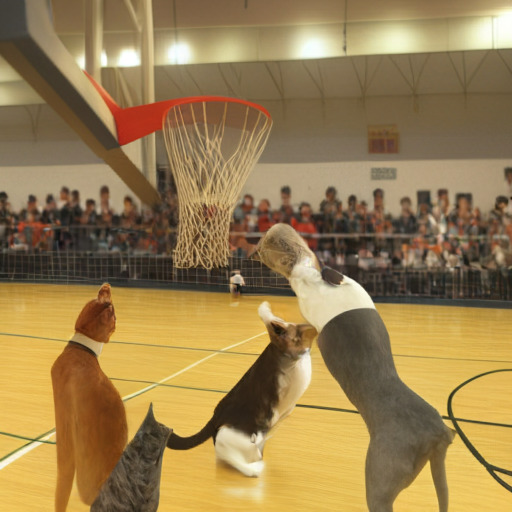
\includegraphics[width=26mm]{figs/failures/failure_00060_maskgit_sresg1r1}
    \\
    \tiny An art gallery displaying Monet paintings. The art gallery is flooded. Robots are going around the art gallery using paddle boards. &
    \tiny A photograph of the inside of a subway train. There are raccoons sitting on the seats. One of them is reading a newspaper. The window shows the city in the background. &
    \tiny Two cups of coffee, one with latte art of yin yang symbol. The other has latter art of a heart. &
    \tiny A cartoon of a dog saying ``I see what you did there''. &
    \tiny Ten wine bottles. &
    \tiny A basketball game between a team of four cats and a team of three dogs.
    \\
  \end{tabular}
  \caption{\small Examples demonstrating text-to-image capabilities of \name~for various text properties. Top left: cardinality; top right: composition; middle left: style; middle right: text rendering; and bottom left: usage of the entire prompt. For all examples, $16$ instances per prompt were generated, and the one with the highest CLIP score \citep{clip} was chosen. Bottom right: examples of generated image failure in \name~for various text properties such as direct rendering of long phrases, high cardinalities, and multiple cardinalities.}
  \label{fig:text_class_examples}
\end{figure}


\renewcommand{\figwidth}{0.93\textwidth}
\begin{figure*}[htbp!]
\vspace{-10pt}
\centering
\captionsetup{width=\figwidth}
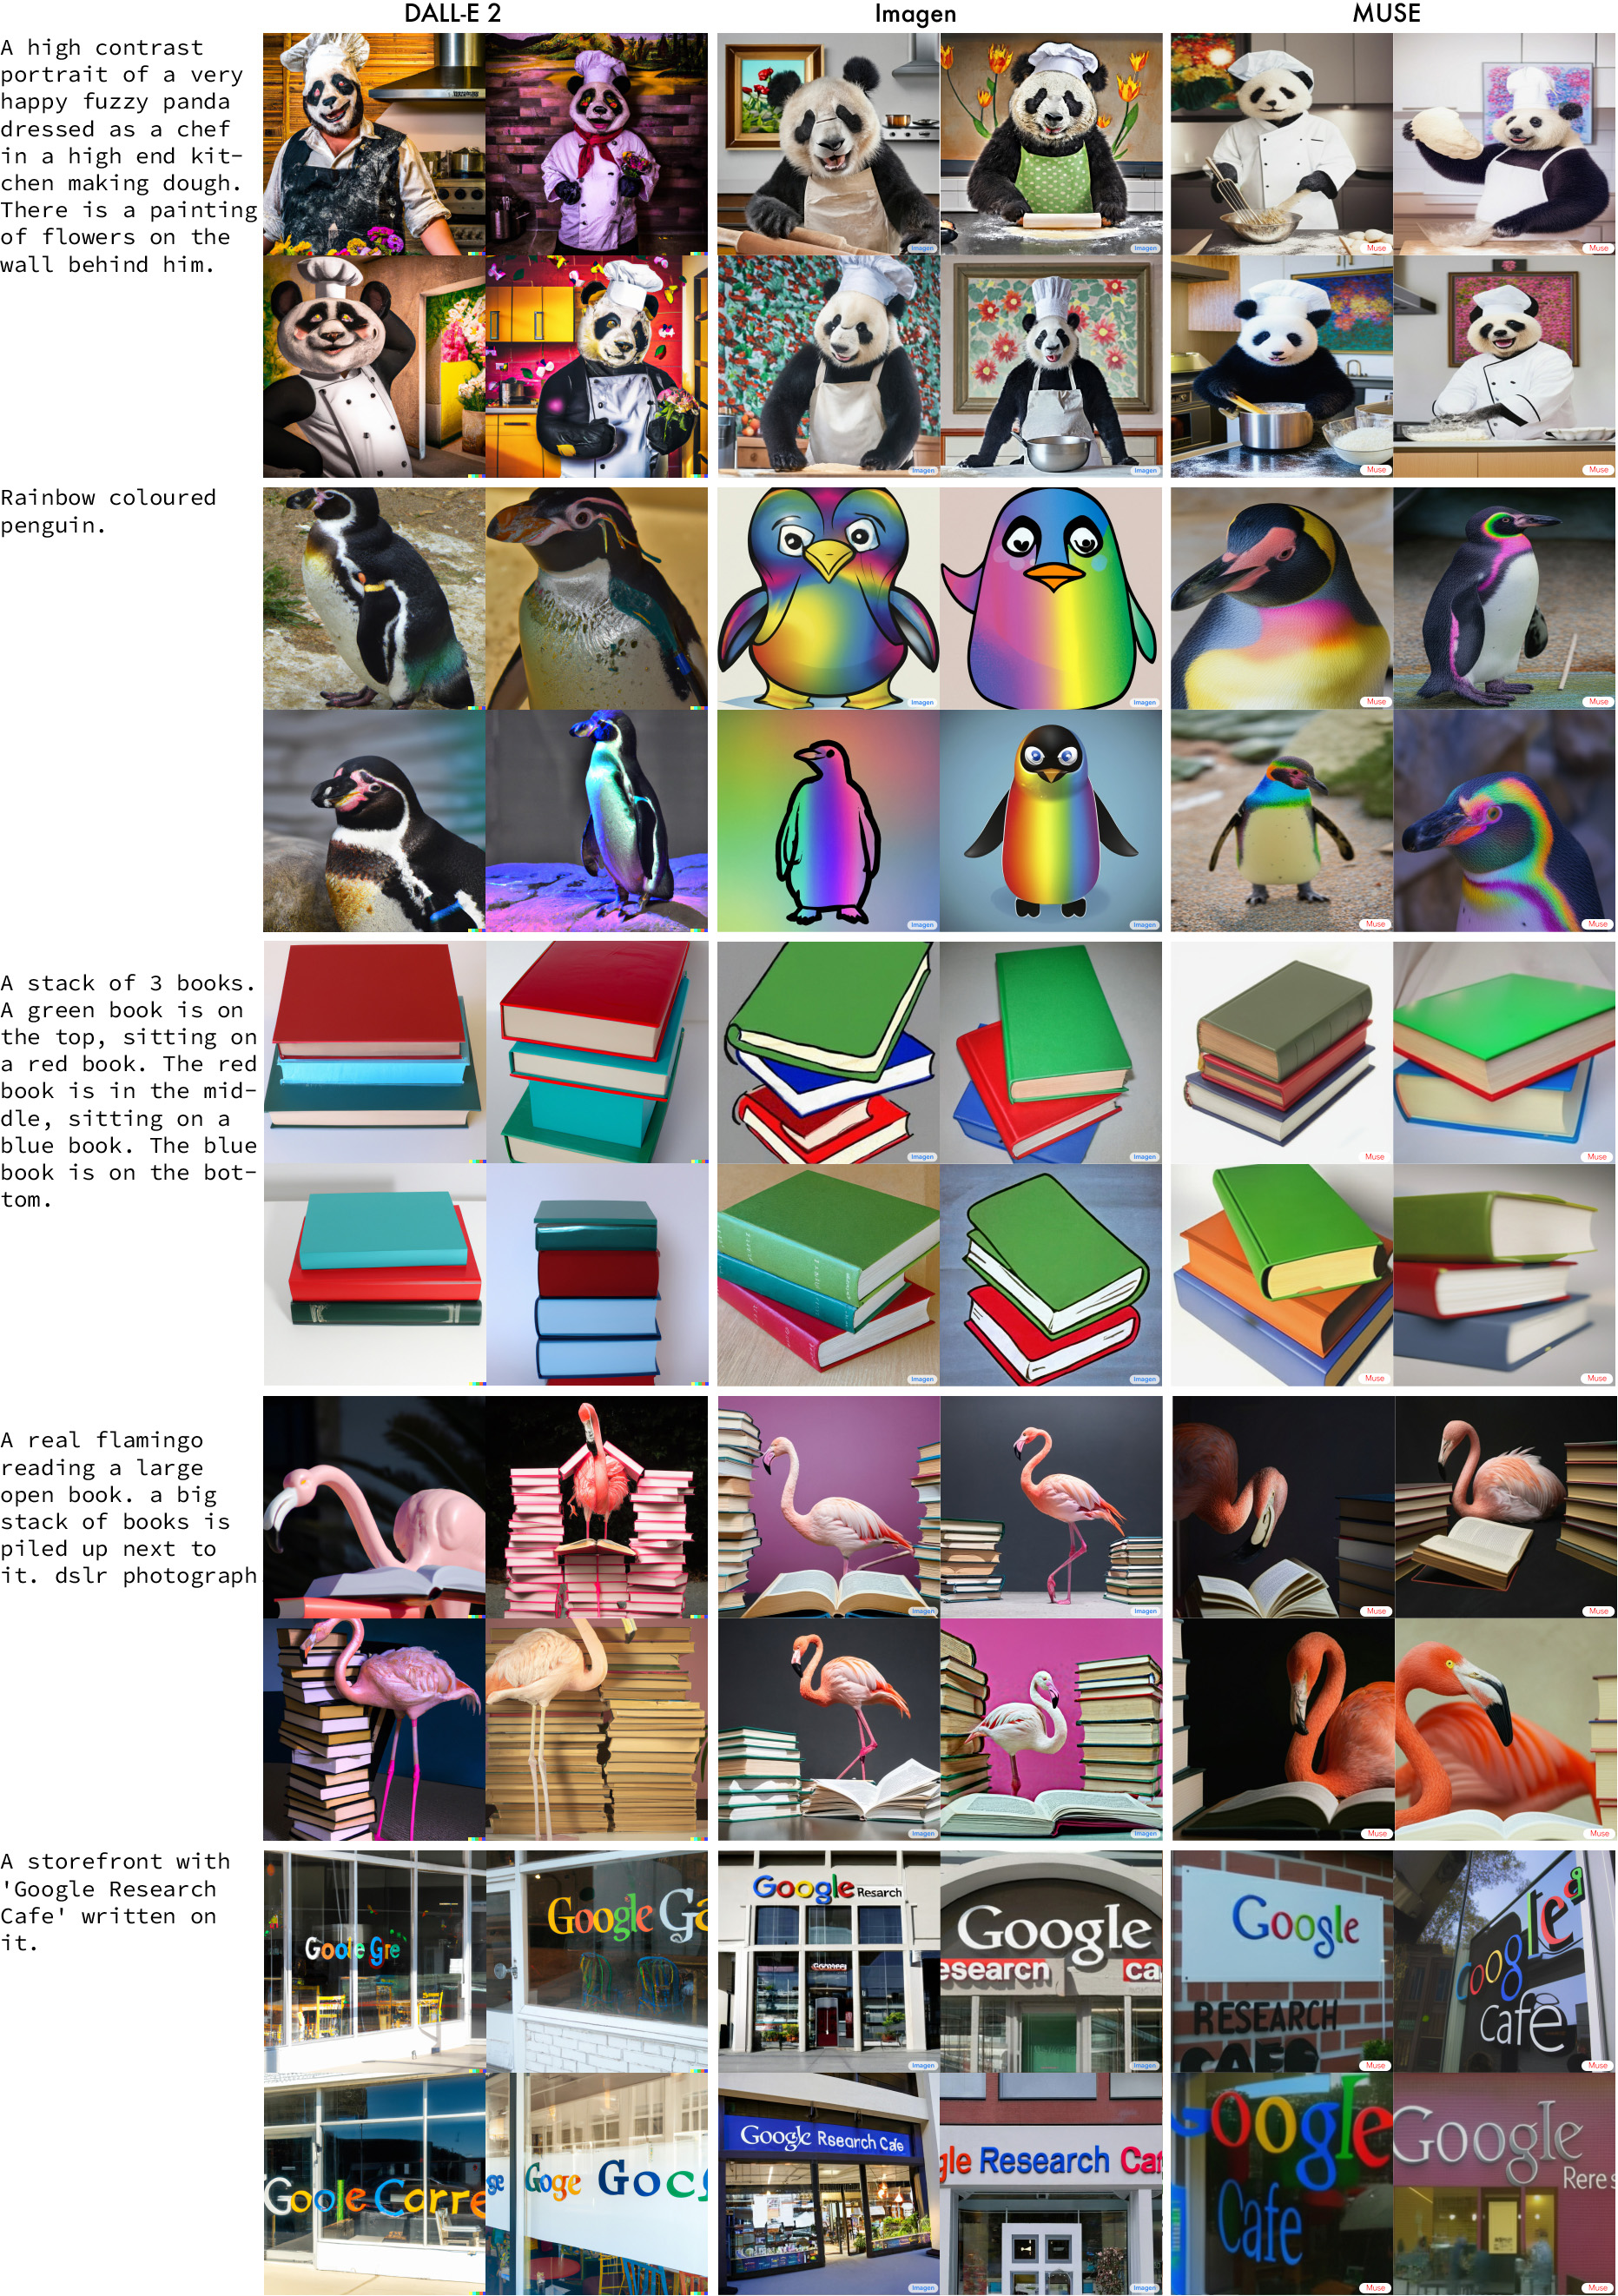
\includegraphics[width=\figwidth]{figs/comparison_muse_watermark}
\vspace{-5pt}
\caption{\small Comparing the same prompts across DALL-E2 \citep{dalle2} (left), Imagen \citep{imagen} (middle) and \name~(right).
}
\vspace{-10pt}
\label{fig:comparison}
\end{figure*}


\subsection{Qualitative Performance}

\figg{text_class_examples} qualitatively demonstrates the capabilities of \name~for text prompts with different properties. The top left of \cref{fig:text_class_examples} shows examples that demonstrate a basic understanding of cardinality. For objects with non-unity cardinality, instead of generating the same object pixels multiple times, \name~instead adds contextual variations to make the overall image more realistic, e.g., elephant size and orientation, wine bottle wrapper color, and tennis ball rotation. The top right of Fig, \ref{fig:text_class_examples} demonstrates understanding of multi-object composition and relativeness. Instead of placing objects at random locations, \name~generates images that preserve prepositional object relations in the text, e.g., on vs under, left vs right, etc. The middle left of \cref{fig:text_class_examples} demonstrates its ability to generate images spanning many styles, both specific to a renowned artist (e.g., Rembrandt) as well as general to a style as a whole (e.g., pop art and Chinese ink and wash). The middle right of \cref{fig:text_class_examples} demonstrates the ability of \name~to render words and phrases. Text generation is fundamentally different than generating most other objects. Instead of the model learning a mapping between an object name and its characteristics (e.g., that ``elephant'' maps to ``large'', ``gray'', and ``peanut eating''), the virtual continuum of possible words and phrases demands that the model learn differently. It must instead learn a hierarchical understanding between phrases, words, and letters. The bottom left of \cref{fig:text_class_examples} demonstrates that \name~uses the entirety of a text prompt when rendering instead of focusing exclusively on only a few salient words. Finally, \cref{fig:comparison} shows comparisons between \name, Dall-E 2 \citep{dalle2}, and Imagen \citep{imagen} for some select prompts, showing that \name~is at par with Imagen and qualitatively better than Dall-E2 for many prompts.

However, as demonstrated in the bottom right of \cref{fig:text_class_examples}, \name~is limited in its ability to generate images well aligned with certain types of prompts. For prompts which indicate that long, multi-word phrases should be directly rendered, ~\name~has a tendency to render those phrases incorrectly, often resulting in (unwanted) duplicated rendered words or rendering of only a portion of the phrase. Additionally, prompts indicating high object cardinality tend to result in generated images which do not correctly reflect that desired cardinality (e.g., rendering only $7$ wine bottles when the prompt specified $10$). In general, the ability of \name~to render the correct cardinalities of objects decreases as the cardinality increases. Another difficult prompt type for \name~is ones with multiple cardinalities (e.g., ``four cats and a team of three dogs''). For such cases, \name~has a tendency to get at least one cardinality incorrect in its rendering.

\subsection{Quantitative Performance}

\begin{table}[t]

\vspace{5pt}
\label{tab:cc3m}
\begin{center}{
  \begin{tabular}{p{50mm} |c | r | r r }
\toprule
 \bfseries{Approach} &
 \bfseries{Model Type} &
 \bfseries{Params} & 
 \bfseries{FID} & 
 \bfseries{CLIP} \\ 
\toprule
VQGAN~\cite{esser2021taming} & Autoregressive &  600M & 28.86 & 0.20 \\
ImageBART~\citep{esser2021imagebart} & Diffusion+Autogressive & 2.8B & 22.61 & 0.23 \\
LDM-4~\citep{ldm} & Diffusion &645M & 17.01 & 0.24 \\
RQ-Transformer \citep{lee2022autoregressive} & Autoregressive & 654M & 12.33 & 0.26 \\
Draft-and-revise \citep{lee2022draft} & Non-autoregressive  & 654M & 9.65 & 0.26 \\
%\tablefootnote{it is a combination of non-autoregressive and autoregressive since the codes in each position is predicted autoregressively.\han{not sure this footnote is needed, I just added to make it precise, but we can totally delete it}}
\midrule
% \rowcolor{LightCyan}
\textbf{\name (base model)} & Non-autoregressive & 632M & 6.8 & 0.25 \\
% \rowcolor{LightCyan}
\textbf{\name (base + super-res)} & Non-autoregressive & 632M + 268M & 6.06 & 0.26 \\
\bottomrule
\end{tabular}
}
\end{center}
\caption{\small Quantitative evaluation on CC3M \citep{sharma2018conceptual}; all models are trained and evaluated on CC3M.}
\label{tab:eval_cc3m}
\vspace{-10pt}
\end{table}

% \parbox{.6\textwidth}{

\begin{table}[t]

\vspace{5pt}
\centering
\label{tab:zero_shot_mscoco}
\begin{tabular}{p{50mm}|c| r | r r}
\toprule
\multirow{2}{*}{\bfseries{Approach}} & \multirow{2}{*}{\bfseries{Model Type}} &
\multirow{2}{*}{\bfseries{Params}} &
\multirow{2}{*}{\bfseries{FID-30K}} &
\bfseries{Zero-shot} \\
& & & & \bfseries{FID-30K} \\
\midrule
AttnGAN \citep{attngan} & GAN & & 35.49 & - \\
DM-GAN \citep{zhu2019dm} & GAN & & 32.64 & - \\
DF-GAN \citep{dfgan} &  GAN & & 21.42 & - \\
DM-GAN + CL \citep{dmgan-cl} &  GAN & & 20.79 & - \\
XMC-GAN \citep{zhang2021cross} & GAN & & 9.33 & - \\
LAFITE \citep{lafite} & GAN & & 8.12 & - \\
Make-A-Scene \citep{makeascene} & Autoregressive & & 7.55 & -\\
\midrule
DALL-E \citep{dalle1} & Autoregressive & & - & 17.89  \\
LAFITE \citep{lafite} & GAN & & - & 26.94 \\
LDM \citep{ldm}  & Diffusion & & -  & 12.63 \\
GLIDE \citep{glide} & Diffusion & & -  & 12.24 \\
DALL-E 2 \citep{dalle2} & Diffusion & & -  & 10.39 \\
Imagen-3.4B \citep{imagen}  & Diffusion & & -  & 7.27 \\ % eyeballed from Figure 4, took highest clip corresponding to the lowest FID

Parti-3B \citep{parti} & Autoregressive & & -  & 8.10 \\
Parti-20B \citep{parti} & Autoregressive & & 3.22  & 7.23\\
\midrule
% \rowcolor{LightCyan}
\textbf{\name-3B} & Non-Autoregressive & & - & \cocofid \\
\bottomrule
\end{tabular}

\caption{\small Quantitative evaluation of FID and CLIP score (where available) on MS-COCO \citep{coco} for $256\times256$ image resolution. \name~ achieves a CLIP score of 0.32, higher than the score of 0.27 reported in Imagen. Other papers in the table above did not report a CLIP score.}
\label{tab:eval_coco}
\end{table}

\begin{figure}
  \centering
  \begin{tabular}{p{0.4\textwidth}p{0.4\textwidth}}
    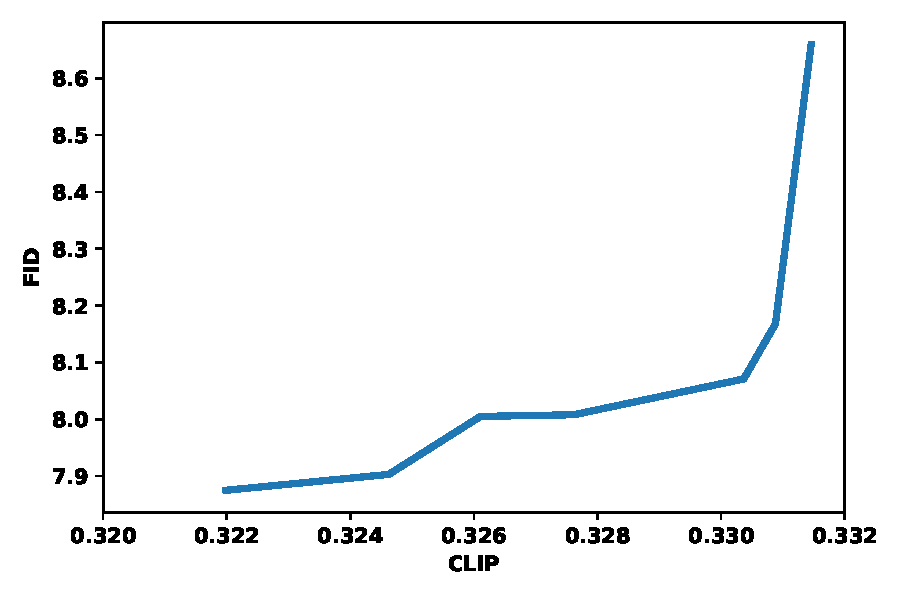
\includegraphics[width=0.4\textwidth,height=0.3\textwidth]{figs/clip_fid}
    \caption{CLIP vs. FID tradeoff curve. We perform sweeps of sampling parameters for a fixed model, then plot the Pareto front.}
    \label{fig:pareto_curve}
    &
    %\vspace{-25pt}
    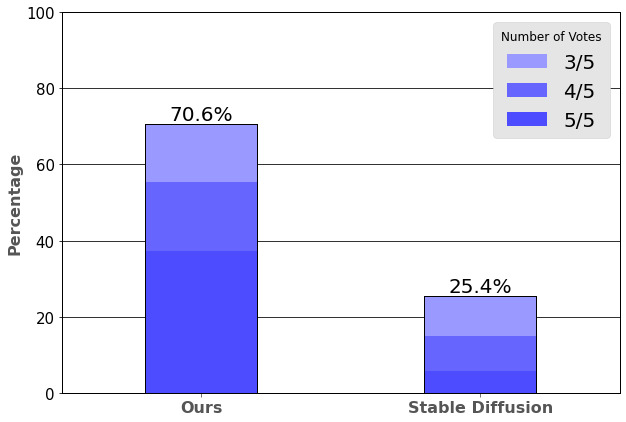
\includegraphics[width=0.4\textwidth,height=0.3\textwidth]{figs/rater_percentages_w_all_labels}
    \caption{\small Percentage of prompts for which a human rater consensus chose a model alignment preference. Contributions from specific numbers of rater consensuses are shown in different colors, while marginals over consensuses ($=\!5$, $\geq4$, and $\geq3$) are shown numerically.}
    %\vspace{-20pt}
    \label{fig:rater_percentages}
  \end{tabular}
\end{figure}

In \tabb{eval_cc3m} and \tabb{eval_coco}, we show our performance against other methods on the CC3M \citep{sharma2018conceptual} and COCO \citep{coco} datasets as measured by Fréchet Inception Distance (FID) \citep{fid}, which measures quality and diversity of samples, as well as CLIP \citep{clip} score, which measures image/text alignment. For the CC3M results, both \name~ models were trained on CC3M. The COCO results are zero-shot, using a model trained on the same dataset as Imagen \citep{imagen}. 

Our 632M model achieves SOTA results on CC3M, significantly improving upon the state of the art in FID score, and also achieving state of the art CLIP score. Our 3B model achieves an FID score of \cocofid~which is slightly better than the score of $8.1$ achieved by the Parti-3B model which has a similar number of parameters. Our CLIP score of \cococlip~is higher than the CLIP score of 0.29 achieved by Imagen (which is achieved when the FID is significantly higher ~20). For the FID of 7.27, Imagen achieves a CLIP score of around 0.27 (see Figure 4 in \citep{imagen}).

Our sampling algorithm (\cref{sec:iterativedec}) has a number of hyperparameters, such as guidance scale, sampling temperature, whether or not to linearly increase guidance during sampling, etc. We perform evaluation sweeps over these parameters. We find subsets of sampling parameters that are Pareto efficient, in the sense that we cannot improve FID without hurting CLIP. This allows us to study the tradeoff between diversity and image/text alignment, which we show in \cref{fig:pareto_curve}.

\subsubsection{Human evaluation}

Similar to previous works \citep{parti, imagen}, we perform side-by-side evaluations in which human raters are presented with a text prompt and two images, each generated by a different text-to-image model using that prompt. The raters are asked to assess prompt-image alignment via the question, ``Which image matches with the caption better?'' Each image pair is anonymized and randomly ordered (left vs right). Raters have the option of choosing either image or that they are indifferent\footnote{Choosing indifference makes sense when neither image is aligned with the text prompt and helps reduce statistical noise in the results.}. Each (prompt, image pair) triplet is assessed by five independent raters; the raters were provided through the Google internal crowd computing team and were completely anonymous to the \name~team. For the set of prompts presented to raters, we used PartiPrompts \citep{parti}, a collection of $1650$ text prompts curated to measure model capabilities across a variety of categories. For the two text-to-image models, we compared \name~($3$B parameters) to that of Stable Diffusion v1.4 \citep{ldm}, the text-to-image model most comparable to \name~in terms of inference speed. For each prompt, $16$ image instances were generated, and the one with the highest CLIP score \citep{clip} was used. The stable diffusion images were generated via the CompVis Stable Diffusion v1.4 notebook \citep{sdgeneration}. We required at least a $3$ rater consensus for results to be counted in favor of a particular model. From this analysis, we found that \name~was chosen as better aligned than Stable Diffusion for $70.6$\% of the prompts, Stable Diffusion was chosen as better aligned than \name~for $25.4$\%, and no rater consensus was chosen for $4$\%. These results are consistent with \name~having significantly better caption matching capability ($\sim\!2.7$x). \cref{fig:rater_percentages} shows a breakdown of the rater results for rater consensuses of $3$, $4$, and all $5$ possible votes. Prompts for which all $5$ raters said \name~had better alignment than Stable Diffusion are the larger contributor.

In addition to measuring alignment, other works \citep{parti, imagen} have also measured image realism, often via a rater question similar to, ``Which image is more realistic?''. However, we note that care must be taken with examination of such results. Though it is not the intent of the question, a model that is completely mode collapsed so that it generates the same sufficiently realistic image regardless of prompt will virtually always do better on this question than a model that \textit{does} take the prompt into account during image generation. We propose this type of question is only applicable between models of similar alignment. Since \name~is significantly better aligned than Stable Diffusion, we did not assess realism via human raters. We consider this topic an area of open research.
\newcommand{\pz}{\hphantom{0}}
\begin{wraptable}{R}{0.5\textwidth}
    \vspace{-30pt}
    \centering
    \begin{tabular}{c|c|r}
         \textbf{Model} & \textbf{Resolution} & \textbf{Time}  \\
         \hline
        %  Imagen (2.3B) & $64\times64$ & TPUv4 & 7s \\
         Imagen & \lowressq &  9.1s \\
         Imagen & $1024\times 1024$ &  13.3s \\
         %LDM (1B), TPUv4 & $512\times 512$ &  7.4s \\
         LDM (50 steps) & $512\times 512$ & 3.7s \\
         LDM (250 steps) & $512\times 512$ & 18.5s \\
         Parti-3B& $256\times256$ & 6.4s \\
         \hline
         \name-3B& \lowressq & 0.5s \\
         \name-3B& \highressq & 1.3s \\
    \end{tabular}
    \vspace{-5pt}
    \caption{\small Per-batch inference time for several models. Muse, Imagen, and Parti were benchmarked internally on TPUv4 hardware. Stable Diffusion/LDM benchmark from \cite{sdinference}, on A100 GPUs. The ``LDM (250 steps)'' time comes from scaling the 50-step time by 5; 250 steps were used to achieve the FID in \cref{tab:eval_coco}.}
    \label{tbl:speed}
    % \begin{tabular}{c|c|c|r}
    %      \textbf{Model (Params)} & \textbf{Resolution} & \textbf{Hardware} & \textbf{Time/image}  \\
    %      \hline
    %     %  Imagen (2.3B) & $64\times64$ & TPUv4 & 7s \\
    %      Imagen (2.9B) & \lowressq & TPUv4 & 9.0s \\
    %      Imagen (3.4B) & $1024\times 1024$ & TPUv4 & 13.0s \\
    %      Stable Diffusion v1.4 (1B) & $512\times 512$ & TPUv4 & 7.4s \\
    %      Stable Diffusion v1.4 (1B) & $512\times 512$ & A100 & 3.7s \\
    %      \hline
    %      \name ~(3B) & \lowressq & TPUv4 & 0.47s \\
    %      \name ~(3B) & \highressq & TPUv4 & 1.3s \\
    % \end{tabular}
    % \vspace{-20pt}
\end{wraptable}

%\yz{If we can get a speed number for Stable Diffusion using TPUv4, then we can replace the A100 number with that.}
\subsubsection{Inference Speed}
\label{sec:speed}
In \cref{tbl:speed}, we compare the inference time of \name~to several other popular models. We benchmarked Parti-3B, Imagen, and Muse-3B internally on TPUv4 accelerators. 
For Stable Diffusion/LDM, we used the fastest reported benchmark \cite{sdinference}, which was done on A100 GPUs. For Stable Diffusion, the TPU implementations we tested were not faster than the A100 implementation. We also report an inference time for LDM with 250 iterations, which is the configuration used to achieve the FID in \cref{tab:eval_coco}. \name~is significantly faster than competing diffusion or autoregressive models, despite having comparable parameter counts (and around 3x more parameters than Stable Diffusion/LDM). The speed advantage of \name~over Imagen is due to the use of discrete tokens and requiring fewer sampling iterations. The speed advantage of \name~over Parti is due to the use of parallel decoding. The speed advantage of \name~over Stable Diffusion is primarily attributable to requiring fewer sampling iterations. 
\subsection{Image Editing}
\label{sec:editing}
By exploiting the fact that our model can condition on arbitrary subsets of image tokens, we can use the model out-of-the-box for a variety of image editing applications with no additional training or model fine-tuning.
\begin{figure*}
  \centering
  \begin{tabular}{p{27mm}p{27mm}p{27mm}p{27mm}p{27mm}}
    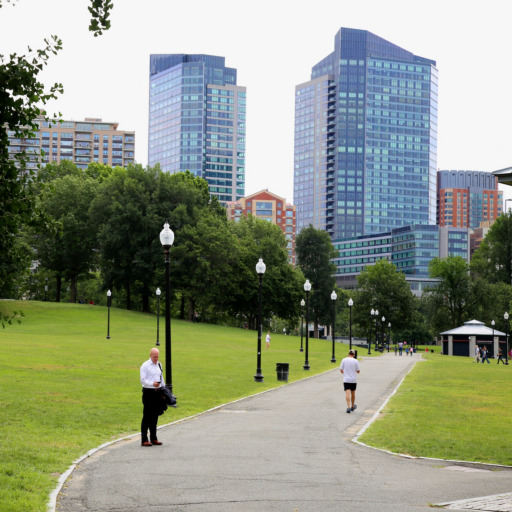
\includegraphics[width=30mm]{figs/inpaint/15_orig} &
    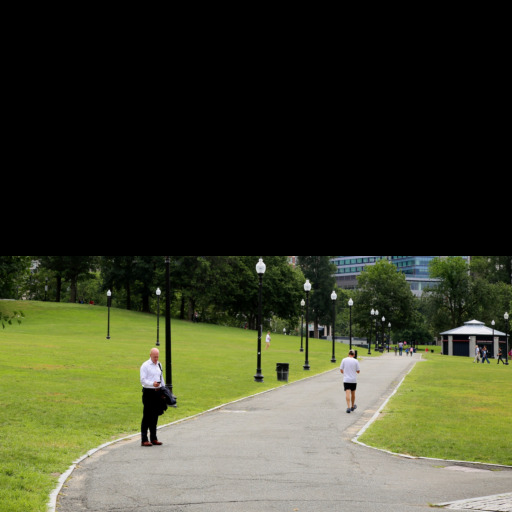
\includegraphics[width=30mm]{figs/inpaint/15_masked} &
    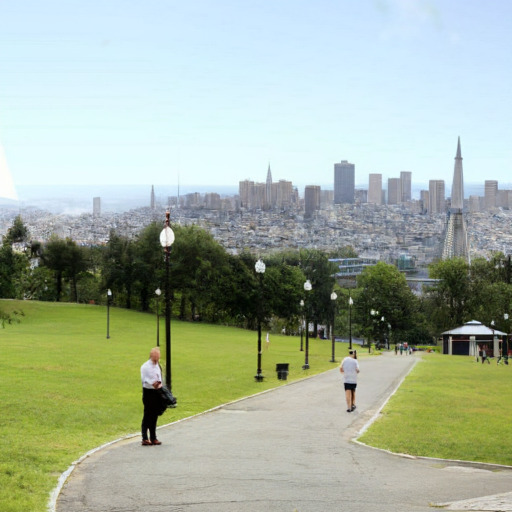
\includegraphics[width=30mm]{figs/inpaint/14_synth_07} &
    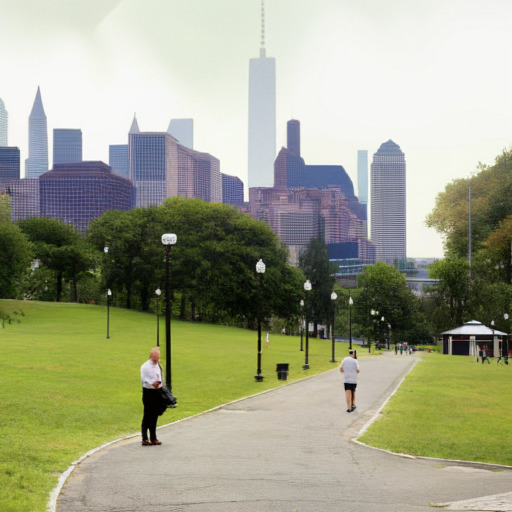
\includegraphics[width=30mm]{figs/inpaint/12_synth_00} &
    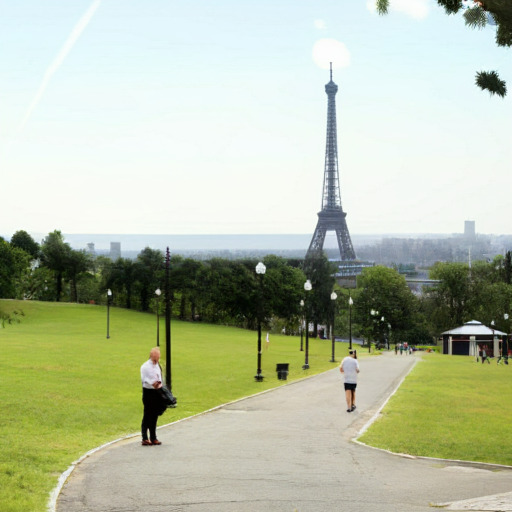
\includegraphics[width=30mm]{figs/inpaint/15_synth_07} 
    \\
     Original &
     Masked &
    {San Francisco in the background} & 
    {New York City in the background} &
    {Paris in the background} 
    \\
    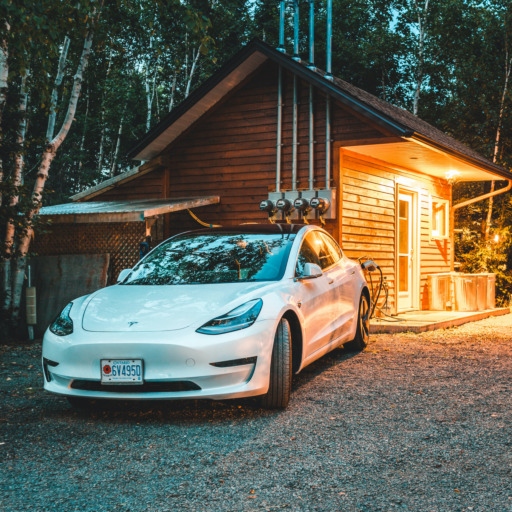
\includegraphics[width=30mm]{figs/inpaint/17_orig} &
    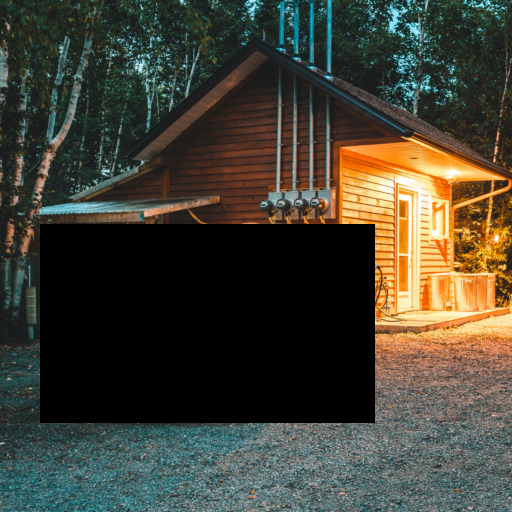
\includegraphics[width=30mm]{figs/inpaint/18_masked} &
    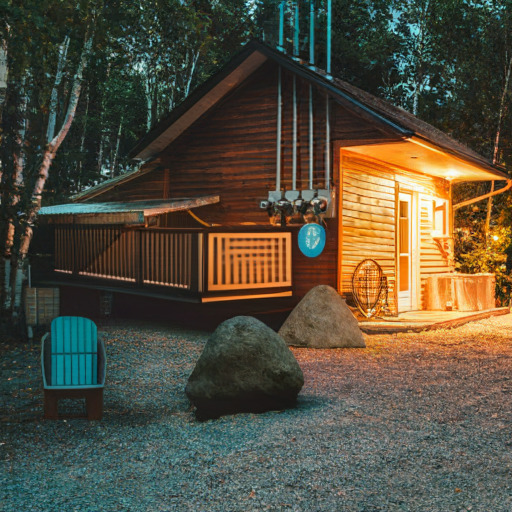
\includegraphics[width=30mm]{figs/inpaint/18_synth_07} &
    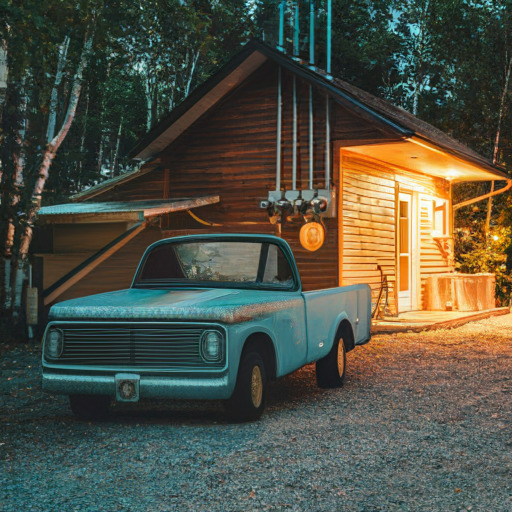
\includegraphics[width=30mm]{figs/inpaint/old_pickup} &
    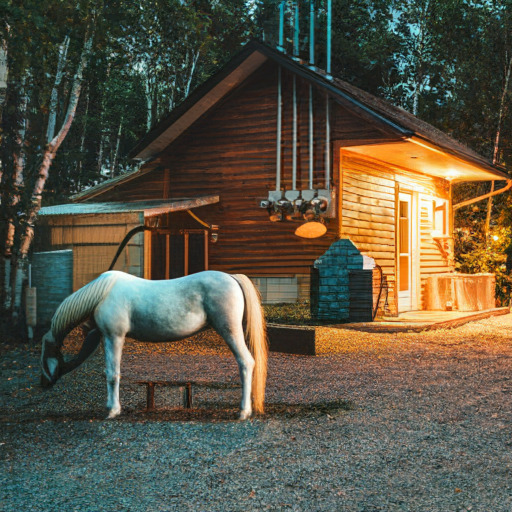
\includegraphics[width=30mm]{figs/inpaint/horse} 
    \\
    Original &
    Masked &
    {A cabin in the woods} & 
    {An old, beat up pickup truck.} & 
    {A horse tied to a post.} 
  \end{tabular}
  \caption{\small Examples of text-guided inpainting. The mask is shown in the second column of each row. This behavior arises directly from the model with no fine-tuning.}
  %\vspace{-30pt}
  \label{fig:inpainting}
\end{figure*}
\subsubsection{Text-guided Inpainting / outpainting}
Our sampling procedure (\cref{sec:iterativedec}) gives us text-guided inpainting and outpainting for free: we convert an input image into a set of tokens, mask out the tokens corresponding to a local region, and then sample the masked tokens conditioned on unmasked tokens and a text prompt. We integrate superresolution through a multi-scale approach: Given an image of size 512x512, we first decimate it to 256x256 and convert both images to high- and low-res tokens. Then, we mask out the appropriate regions for each set of tokens. Next, we inpaint the low-res tokens using the parallel sampling algorithm. Finally, we condition on these low-res tokens to inpaint the high-res tokens using the same sampling algorithm. We show examples of this in \cref{fig:teaser_edit} and \cref{fig:inpainting}.

\subsubsection{Zero-shot Mask-free editing}
We use \name~in a zero-shot sense for mask-free image editing of real input images. This method works directly on the (tokenized) image and does not require ``inverting'' the full generative process, in contrast with recent zero-shot image editing techniques leveraging generative models \citep{gal2022stylegan,patashnik2021styleclip,kim2022diffusionclip,nulltext2022}. 

We first convert an input image into visual tokens. Next, we iteratively mask and resample a random subset of tokens, conditioned on text prompts. We can think of this as being analogous to a Gibbs sampling procedure, where we fix some tokens and resample others conditioned on them. This has the effect of moving the tokenized image into the typical set of the conditional distribution of images given a text prompt. 

We perform the editing using the low-resolution base model, then perform superres on the final output (conditioned on the editing prompt). In the examples (\cref{fig:teaser_edit}, \cref{fig:mfe_gallery}), we resample 8\% of the tokens per iteration for 100 iterations, with a guidance scale of 4. We also perform top-$k$ ($k=3$) sampling on the token logits to prevent the process from diverging too much from the input. The iterative nature allows for control over the final output. \cref{fig:edit_iter} shows a few intermediate edits (without superres); in this example, the user may prefer iteration 50 or 75 over the final output.

\begin{figure*}
  \centering
  \begin{tabularx}{0.95\textwidth}{p{0mm}p{27mm}p{27mm}p{27mm}p{27mm}p{27mm}}
    \rotatebox{90}{\hspace{5mm}Input image} &
    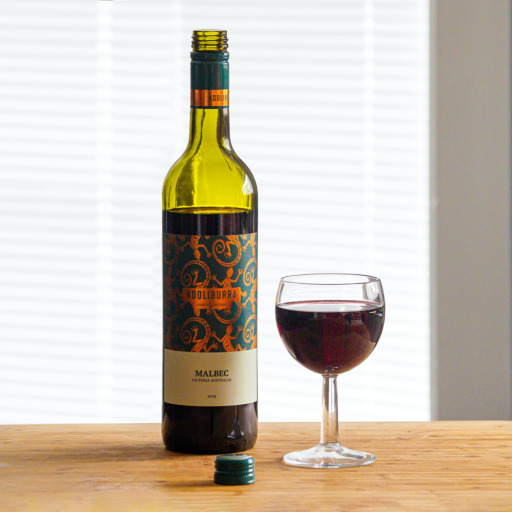
\includegraphics[width=30mm]{figs/mfe/68_seed_1_orig_sr} &
    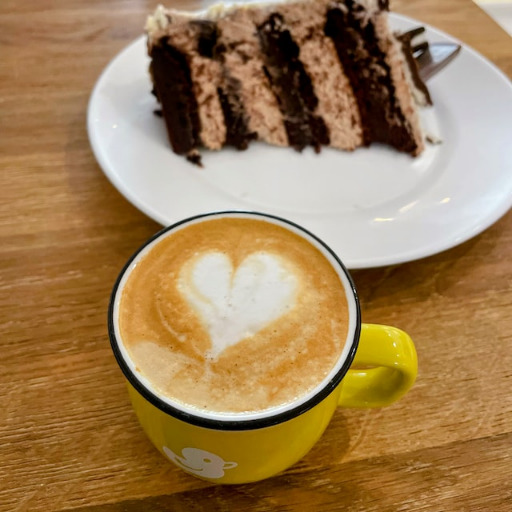
\includegraphics[width=30mm]{figs/mfe/18_seed_0_orig_sr} &
    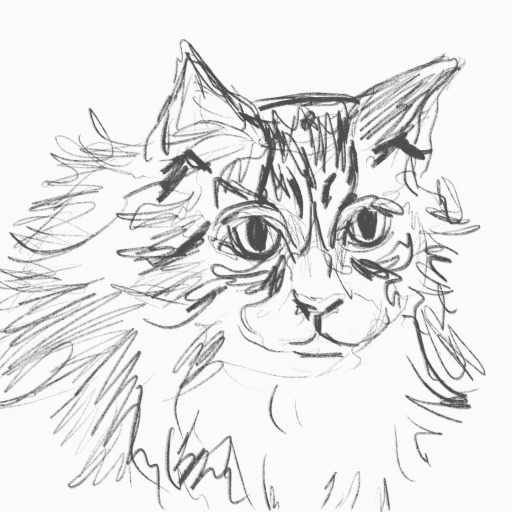
\includegraphics[width=30mm]{figs/mfe/06_seed_6_orig_sr} &
    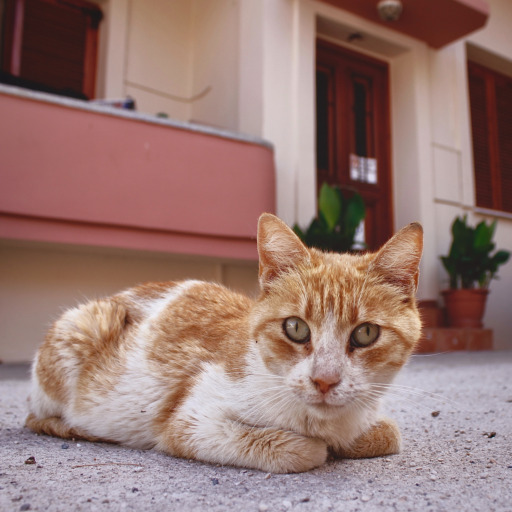
\includegraphics[width=30mm]{figs/mfe/19_seed_2_orig_sr} &
    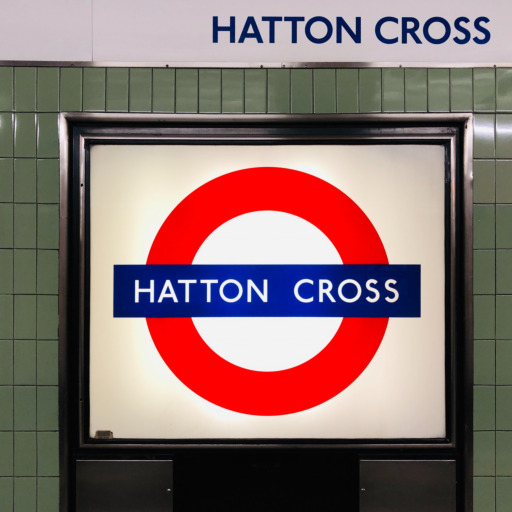
\includegraphics[width=30mm]{figs/mfe/21_seed_3_orig_sr} 
    \\
    \rotatebox{90}{\hspace{5mm}Editing output\vspace{-3mm}} &
    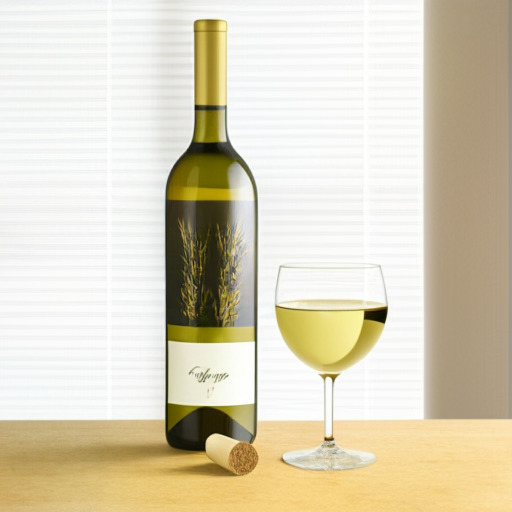
\includegraphics[width=30mm]{figs/mfe/68_seed_1_synth_sr} &
    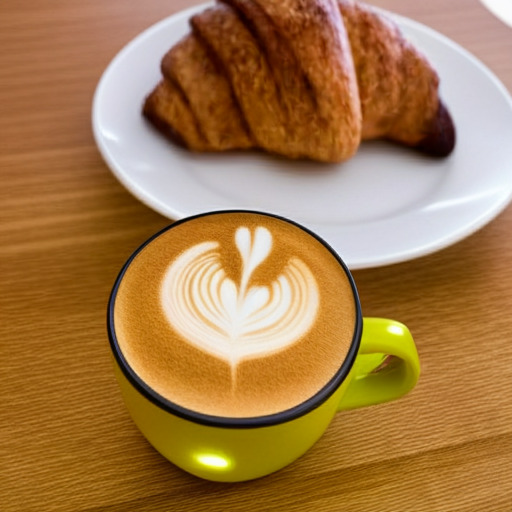
\includegraphics[width=30mm]{figs/mfe/18_seed_0_synth_sr} &
    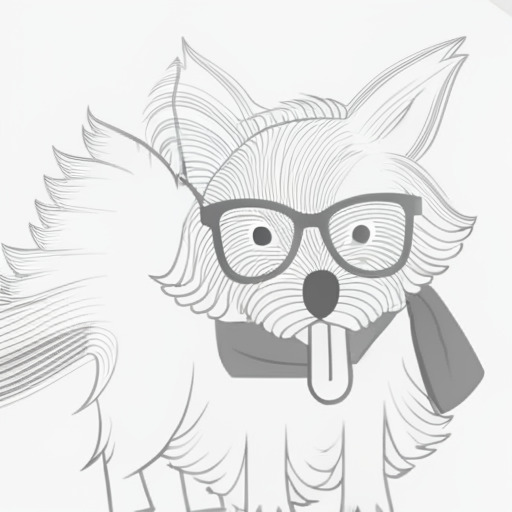
\includegraphics[width=30mm]{figs/mfe/06_seed_6_synth_sr} &
    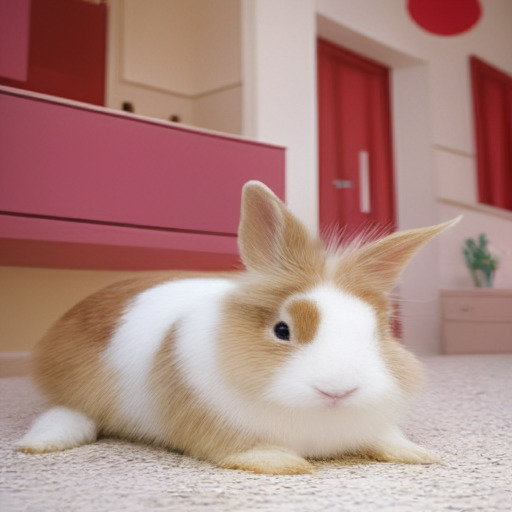
\includegraphics[width=30mm]{figs/mfe/19_seed_2_synth_sr} &
    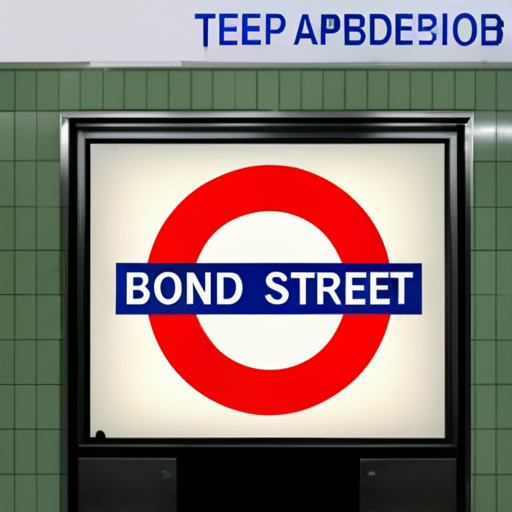
\includegraphics[width=30mm]{figs/mfe/21_seed_3_synth_sr} 
    \\
    &
    A bottle of Pinot Grigio next to a glass of white wine and a cork. &
    A croissant next to a latte with a flower latte art. &
    A dog. &
    A brown rabbit. &
    Bond Street.
    \\
    \rotatebox{90}{\hspace{5mm}Input image} &
    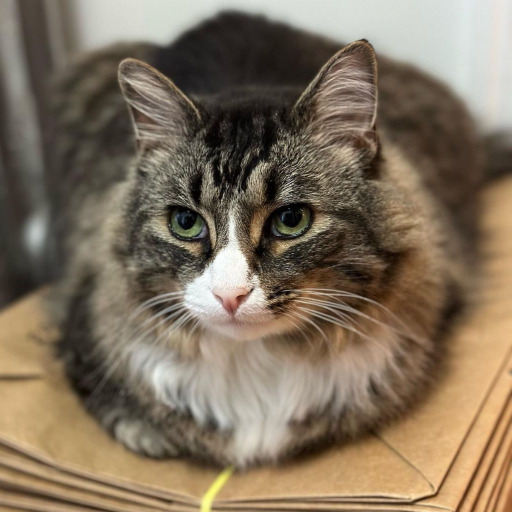
\includegraphics[width=30mm]{figs/mfe/01_seed_0_orig_sr} &
    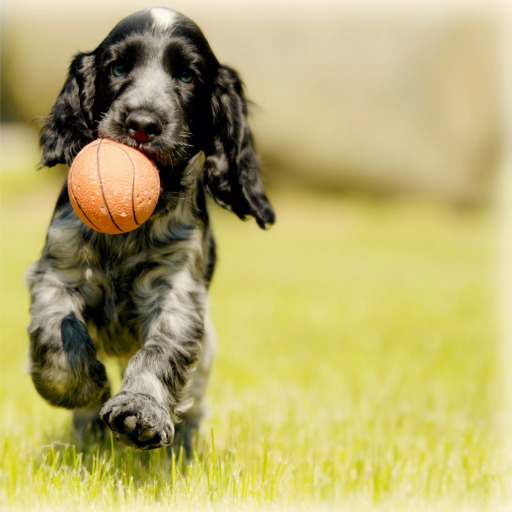
\includegraphics[width=30mm]{figs/mfe/65_seed_7_orig_sr} &
    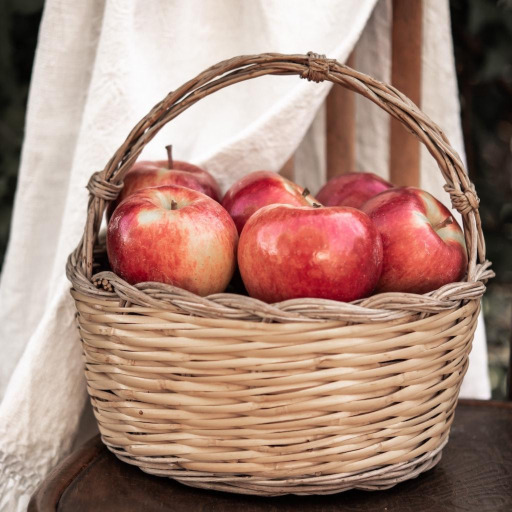
\includegraphics[width=30mm]{figs/mfe/27_seed_2_orig_sr} &
    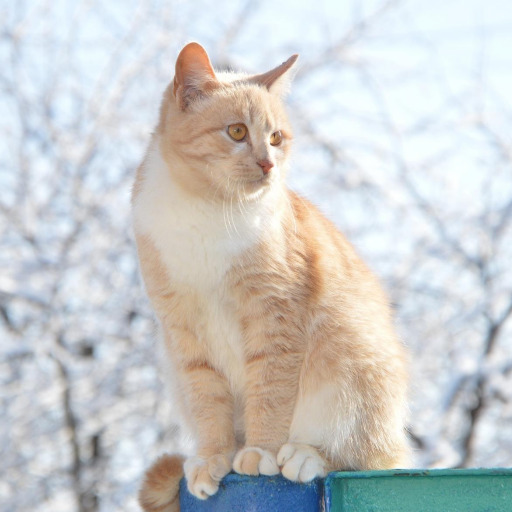
\includegraphics[width=30mm]{figs/mfe/43_seed_7_orig_sr} &
    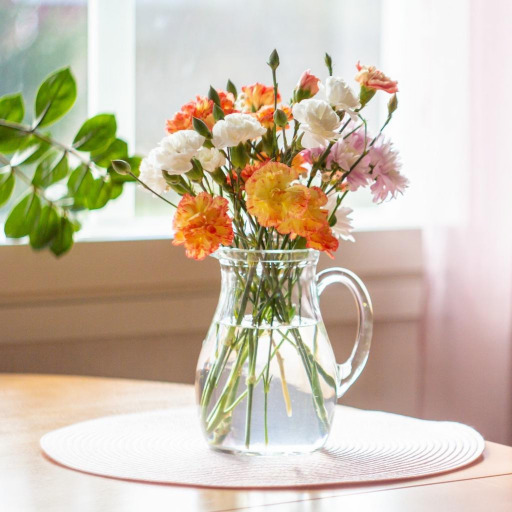
\includegraphics[width=30mm]{figs/mfe/59_seed_6_orig_sr}
    \\
    \rotatebox{90}{\hspace{5mm}Editing output\vspace{-3mm}} &
    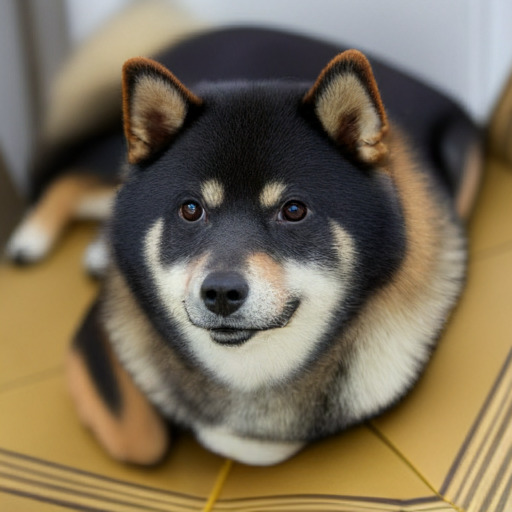
\includegraphics[width=30mm]{figs/mfe/01_seed_0_synth_sr} &
    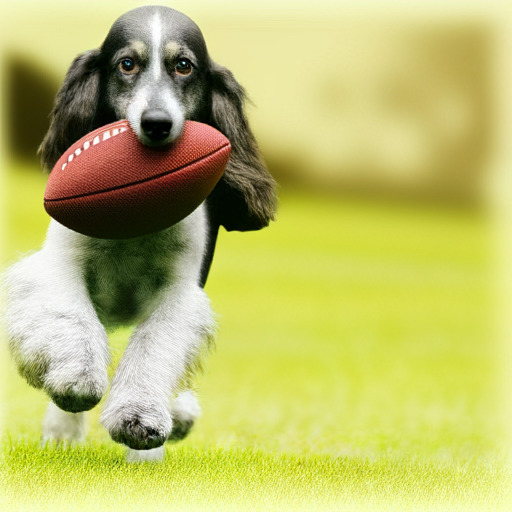
\includegraphics[width=30mm]{figs/mfe/65_seed_7_synth_sr} &
    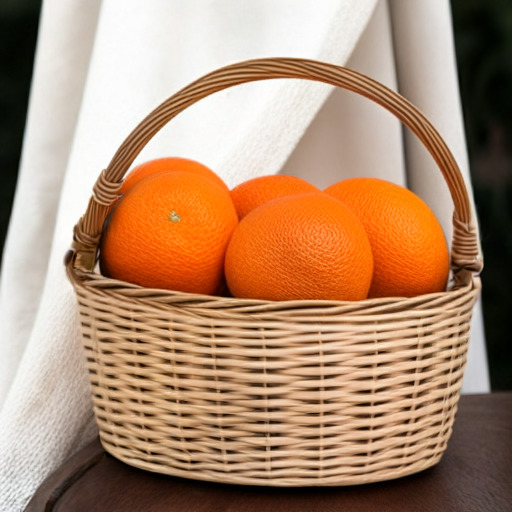
\includegraphics[width=30mm]{figs/mfe/27_seed_2_synth_sr} &
    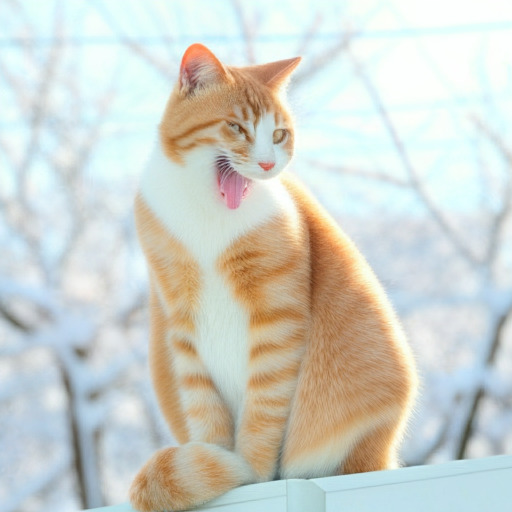
\includegraphics[width=30mm]{figs/mfe/43_seed_7_synth_sr} &
    \includegraphics[width=30mm]{figs/mfe/59_seed_6_synth_sr} 
    \\
    &
    A Shiba Inu&
    A dog holding a football in its mouth &
    A basket of oranges&
    A photo of a cat yawning&
    A photo of a vase of red roses
  \end{tabularx}
  \caption{Examples of zero-shot mask-free image editing, post superres. We see that the pose and overall structure of the image is maintained while changing some specific aspects of the object based on the text prompt.}
  \label{fig:mfe_gallery}
\end{figure*}


\begin{figure*}
    \centering
  \begin{tabular}{p{0.95\textwidth}}
  \hspace{5mm}
    \includegraphics[width=150mm]{figs/mfe/18_seed_0_timeline}\\ 
    \hspace{5mm}
    \begin{tabularx}{150mm}{p{25mm}p{25mm}p{25mm}p{25mm}p{25mm}}
    Input  &
    Iteration 25 &
    Iteration 50 &
    Iteration 75 &
    Iteration 100
    \end{tabularx}
  \end{tabular}
    \caption{Intermediate iterations producing one of the edits in \cref{fig:mfe_gallery} (pre-superres)}
    \label{fig:edit_iter}
\end{figure*}

